\section{Results}
Before any improvements the system had a probability of failure P(F)= 0,71. After improvements we have removed F0 and F9 from the general fault tree, and F2, F3 from the destructive fault tree (F8) and the probability of failure is reduced to P(F)= 0,18. The updated fault trees are shown in \cref{fig:ftree_drsstc_dest_i} and \cref{fig:ftree_drsstc_i}. The probability for destructive failure P(F8) is reduced from 0,666 to 0,096.


\begin{figure}[h]
\begin{circuitikz}[scale = 0.7, transform shape] \draw
(0,0) node[] (x0){F7: Limiter settings}
(0,1.2) node[] (x1){F6: Limiter def.}
(0,2.2) node[] (x2){F5: Sig. gen settings}
(0,2.8) node[] (x3){F4: Sig. gen def.}
%(0,4) node[] (x4){F3: Optical cable missing}
%(0,5) node[] (x5){F2: Optical cable def.}
(0,4) node[] (x6){F1: CW detection def.}
%(0,7) node[] (x7){F0: HV cables disconnected}
(13,2) node[] (x8){F8: Destructive failure}
%(4,6.5) node[or port] (myor1) {}
%(4,4.5) node[or port] (myor2) {}
(4,2.5) node[or port] (myor3) {}
(6,1.5) node[and port] (myand1) {}
%(8,2.5) node[or port] (myor4) {}
(8,3) node[and port] (myand2) {}
(10,2) node[or port] (myor5) {}
(x0) -- (8,0) -- (myor5.in 2)
(x1) -- (myand1.in 2)
(x2) -- (myor3.in 2)
(x3) -- (myor3.in 1)
%(x4) -- (myor2.in 2)
%(x5) -- (myor2.in 1)
%(x6) -- (myor1.in 2)
%(x7) -- (myor1.in 1)
(myor5.out) -- (x8)
(x6) -- (6,4) -- (myand2.in 1)
%(myor2.out) -- (myor4.in 1)
(myor3.out) -- (myand1.in 1)
%(myand1.out) -- (myor4.in 2)
(myand1.out) -- (myand2.in 2)
(myand2.out) -- (myor5.in 1);
\end{circuitikz}
\caption{Fault tree for destructive failure of DRSSTC}
    \label{fig:ftree_drsstc_dest_i}
\end{figure}

\begin{figure}[h]
\begin{circuitikz} \draw
(0,1) node[] (x0){F8: Destructive failure}
%(0,1) node[] (x1){F9: Internal cables missing}
(0,0) node[] (x2){F2: Optical cable defective}
(8,0.5) node[] (x3){Failure}
(6,0.5) node[or port] (myor1) {}
%(6,1.5) node[or port] (myor2) {}
%(x0) -- (myor2.in 1)
(x1) -- (myor1.in 1)
(x2) -- (myor1.in 2)
(myor1.out) -- (x3);
\end{circuitikz}
\caption{Fault tree for non-destructive failure of DRSSTC}
    \label{fig:ftree_drsstc_i}
\end{figure}

In \cref{fig:TK530_before} the power amplifier with and without back plane is shown


\begin{figure}
    \centering
    \begin{subfigure}{0.45\textwidth}
        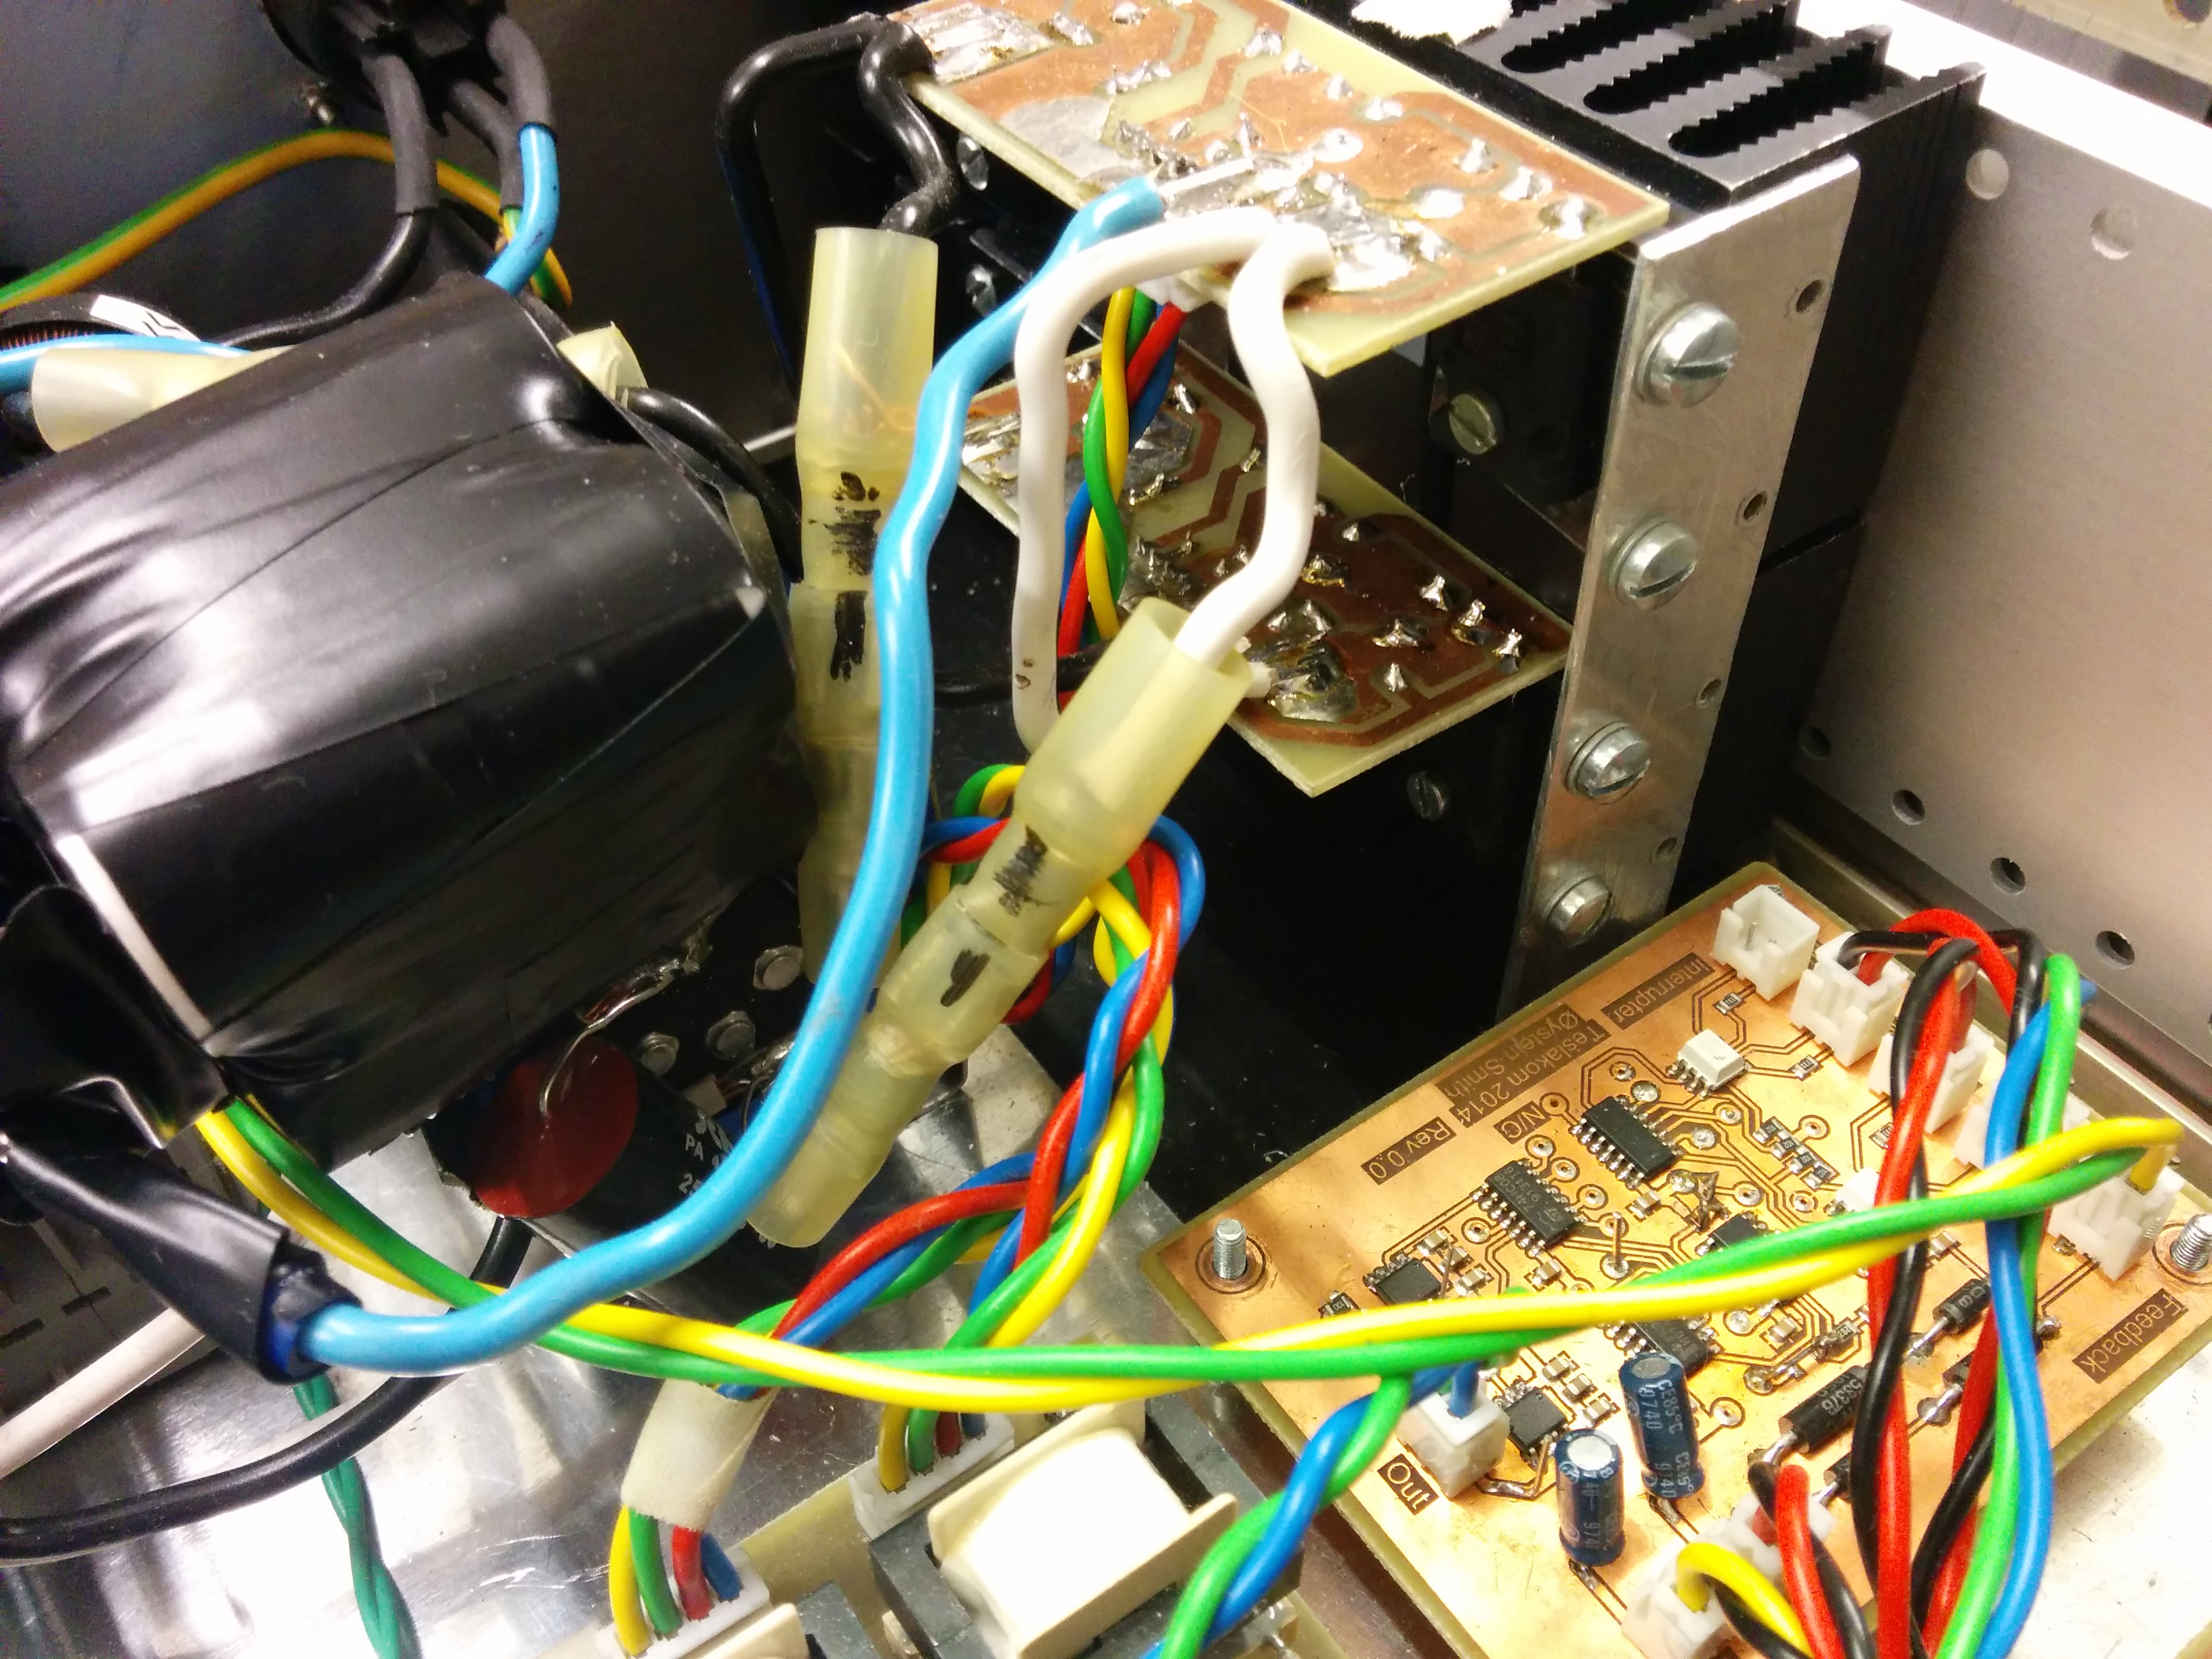
\includegraphics[width=0.8\textwidth]{img/IMG_20161212_162711.jpg}
        \caption{Power amplifier without back plane}
        \label{fig:TK530_before}
    \end{subfigure}
    ~
    \begin{subfigure}{0.45\textwidth}
        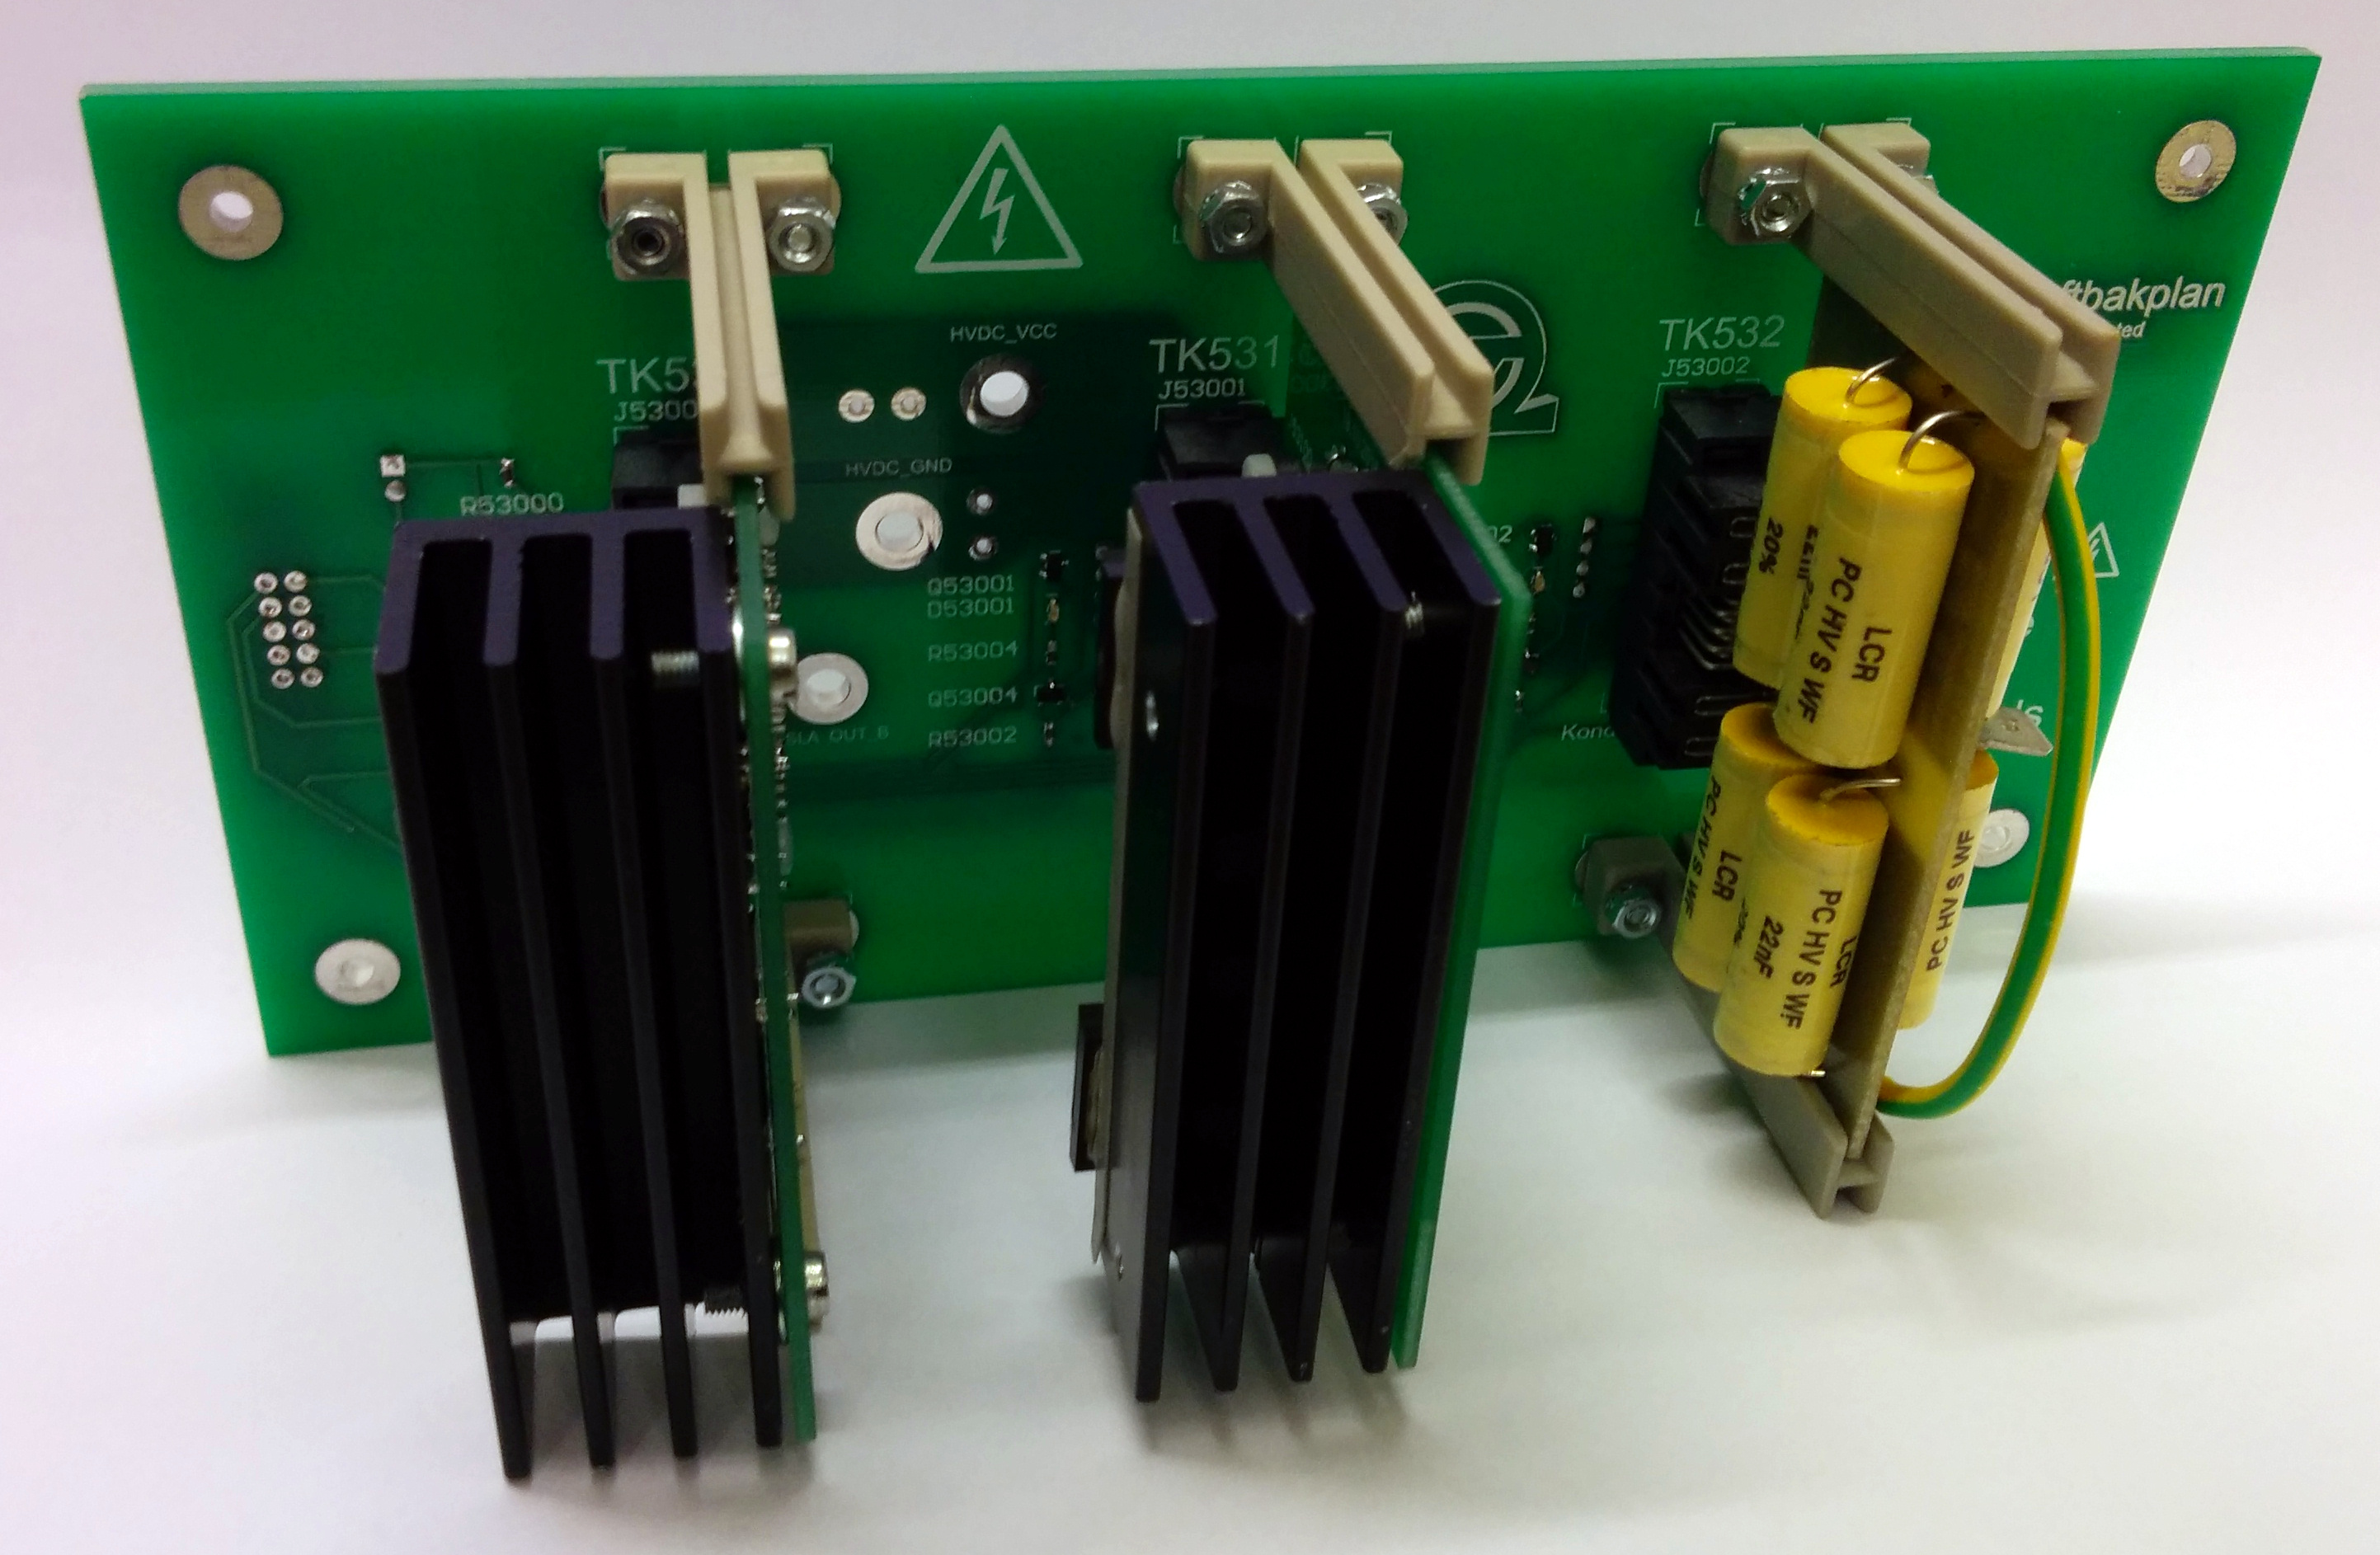
\includegraphics[width=0.8\textwidth]{img/TK530_Kraftbakplan.jpg}
        \caption{Power amplifier with back plane}
        \label{fig:TK530_after}
    \end{subfigure}
\end{figure}